Using the scalar product
\begin{align}
  \cos{60\degree}=
\frac{1}{2}=\frac{\myvec{
        1&2
    }\myvec{
        1\\m
    }}{\sqrt{5}\sqrt{m^2+1}}\\
\implies 11m^2+16m-1=0\\
   or, m=\frac{-8\pm5\sqrt{3}}{11}    
\end{align}
So, the desired equation of the line is
\begin{align}
\myvec{
    \frac{-8\pm5\sqrt{3}}{11}&-1
}\vec{x} 
	&=
\myvec{
    \frac{-8\pm5\sqrt{3}}{11}&-1
}
\myvec{
    2\\3}
    \\
	&=\frac{-49\pm16\sqrt{3}}{11}
\end{align}
\iffalse
See 
    \figref{fig:11.10.3.12}.
\begin{figure}[H]
    \centering
    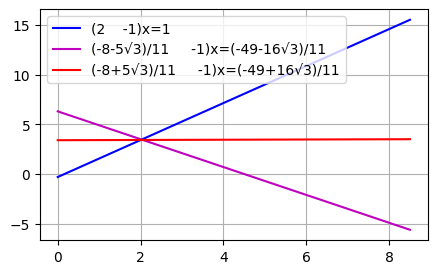
\includegraphics[width=0.75\columnwidth]{chapters/11/10/3/12/fig/asgnt1.png}
    \caption{}
    \label{fig:11.10.3.12}
\end{figure}
\fi

